\documentclass[10pt]{article}

\usepackage[top=2cm,bottom=2cm,right=2cm,left=2cm]{geometry}
\usepackage{fancyhdr}
\usepackage{amsmath,amsthm,amssymb,amsfonts}
\usepackage{listings}
\usepackage{graphicx,subfig}

\fancyhead[L]{\textbf{Lucas E. Quintero}}
\fancyhead[C]{\textbf{Homework1}}
\fancyhead[R]{\textbf{\today}}
\fancyfoot[L]{MATH598B}
\fancyfoot[C]{}
\fancyfoot[R]{\thepage}

\pagestyle{fancy}

\begin{document}
\begin{description}
\item[Problem 1]\hfill\\
The R function to find the mean and standard deviation is
\begin{lstlisting}[frame=trBL]
#Function for Problem 1
#Purpose is to find mean and standard deviation of all columns
#Mean is stored in column 1 of output
#Standard Deviation is stored in column 2 of output

Problem1Fun<-function(InTable){
	OutVec<-matrix(c(1:2*dim(InTable)[2]),ncol=2,nrow=dim(InTable)[2])
	for(i in 1:dim(InTable)[2]){
		OutVec[i,1]<-mean(InTable[,i])
		OutVec[i,2]<-sd(InTable[,i])
	}
	return(OutVec)
}
\end{lstlisting}
The output for running \verb+Problem1Fun(Nitrates)+ is
\begin{lstlisting}[frame=trBL]
> Problem1Fun(Nitrates)
             [,1]         [,2]
 [1,]     2.00000 1.351725e+00
 [2,]    33.68870 8.366869e-02
 [3,]  -112.21931 3.152602e-01
 [4,]   483.08873 1.128625e+02
 [5,] 37431.11734 1.647951e+04
 [6,]   679.43042 1.093556e+03
 [7,] 26499.28471 1.576737e+04
 [8,]    26.52196 2.216925e+01
 [9,]    17.79275 7.931085e+01
[10,]     7.54878 5.698698e-01
[11,]   613.55278 1.320502e+03
\end{lstlisting}
To use the \verb+apply+ function to produce the means in 1 line, we would use the following command and the output is as follows
\begin{lstlisting}[frame=trBL]
> apply(Nitrates,2,mean)
        LAND.USE.LEVEL1       latitude_decimals       longitude_decimal 
                2.00000                33.68870              -112.21931 
      elevation.Meters. DistanceFromUrbanCenter             POP_DENSITY 
              483.08873             37431.11734               679.43042 
      INCOME_PER_CAPITA                VegCover                   NO3.N 
            26499.28471                26.52196                17.79275 
                     pH            conductivity 
                7.54878               613.55278 
\end{lstlisting}
Similarly, we have the following for standard deviation:
\begin{lstlisting}[frame=trBL]
> apply(Nitrates,2,sd)
        LAND.USE.LEVEL1       latitude_decimals       longitude_decimal 
           1.351725e+00            8.366869e-02            3.152602e-01 
      elevation.Meters. DistanceFromUrbanCenter             POP_DENSITY 
           1.128625e+02            1.647951e+04            1.093556e+03 
      INCOME_PER_CAPITA                VegCover                   NO3.N 
           1.576737e+04            2.216925e+01            7.931085e+01 
                     pH            conductivity 
           5.698698e-01            1.320502e+03 
\end{lstlisting}
\item[Problem 2]\hfill\\
We create a dataframe with rows with a pH value of 7, then plot NO3 against conductivity with the following code and then the output plot is the included
\begin{lstlisting}[frame=trBL]
> pH7Nitrates<-Nitrates[which(Nitrates$pH==7),]
> plot(pH7Nitrates$conductivity,pH7Nitrates$NO3.N,
	main="NO3.N vs Conductivity for pH of 7")
> dev.print(device=pdf,"Problem2.pdf")
\end{lstlisting}
\begin{figure}[h]
{\centering
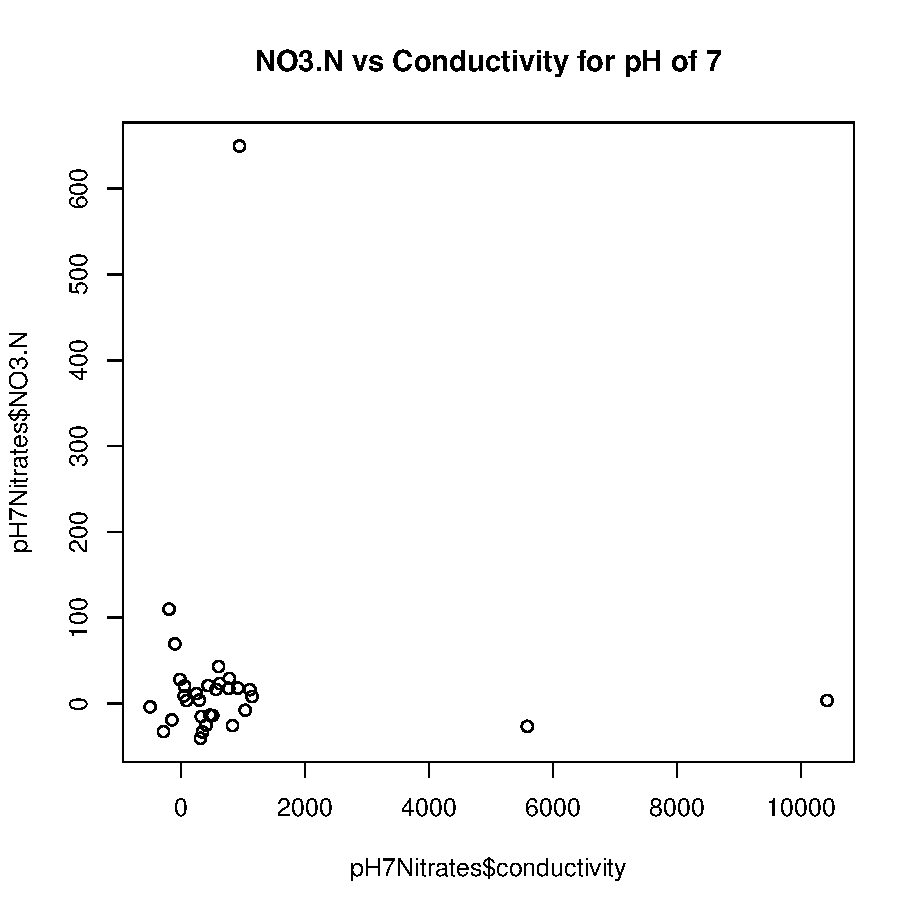
\includegraphics[width=15cm]{../Problem2.pdf}}
\end{figure}
 
\item[Problem 3]\hfill\\
To produce a side-by-side histogram of NO3.N for pH of 7 and pH of 8, we create two dataframes and then use \verb+hist()+ which produces the subsequent plot.
\begin{lstlisting}[frame=trBL]
> pH7Nitrates<-Nitrates[which(Nitrates$pH==7),]
> pH8Nitrates<-Nitrates[which(Nitrates$pH==8),]
> par(mfrow=c(1,2))
> hist(pH7Nitrates$NO3.N)
> hist(pH8Nitrates$NO3.N)
> dev.print(device=pdf,"Problem3.pdf")
\end{lstlisting}
\begin{figure}[ht!]
\centering
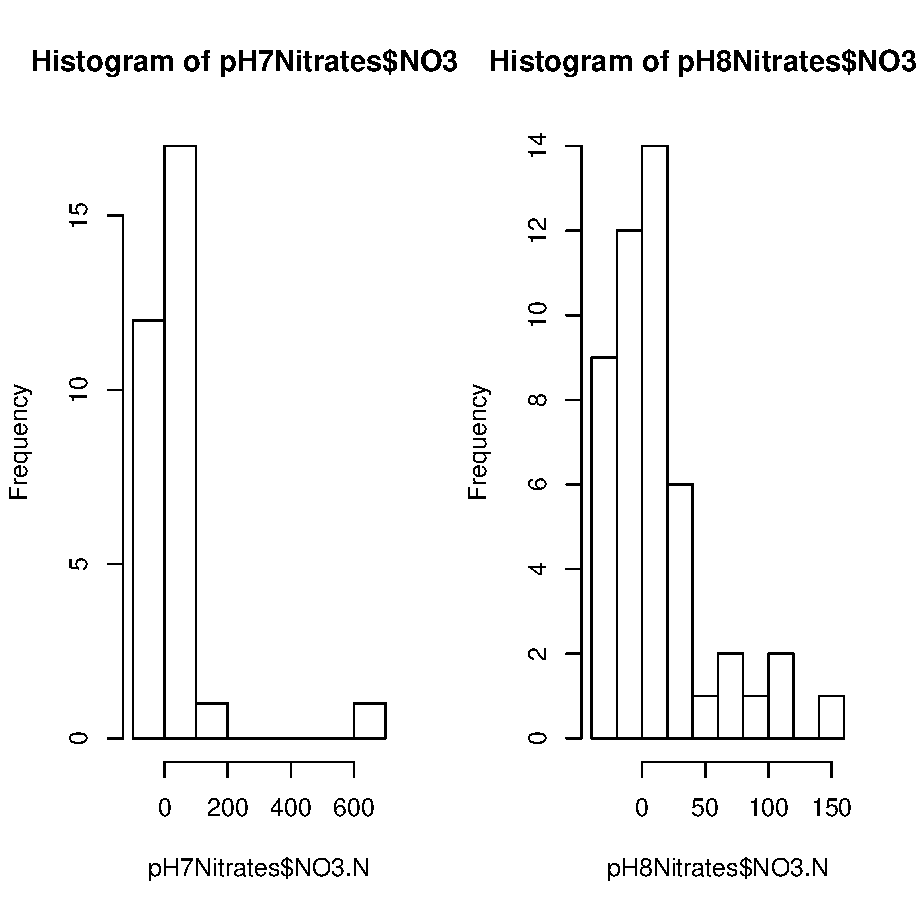
\includegraphics[width=15cm]{../Problem3.pdf}
\end{figure}

\item[Problem 4] \hfill\\
To determine how many data points have a landuse of 2, we use the following line
\begin{lstlisting}[frame=trBL]
> dim(Nitrates[which(Nitrates$LAND.USE.LEVEL1==2),])[1]
[1] 45
\end{lstlisting}
So, we see that there are 45 data points with a landuse of 2.

\item[Problem 5]\hfill\\
After installing packages with \verb+install.packages('mvtnorm')+ then using the following given code
\begin{lstlisting}[frame=trBL]
 library(mvtnorm)

 for(i in 1:1000){
		currentrealization<-rmvnorm(1,c(0,0),CovMat)
		Realizations[i,1]<-currentrealization[1,1]
		Realizations[i,2]<-currentrealization[1,2]
 }
\end{lstlisting}
we can create a covariance matrix with the given values and create a matrix of zeros 
\begin{lstlisting}[frame=trBL]
> CovMat<-matrix(rep(1,4),nrow=2,ncol=2)
> CovMat[1,]<-c(1,0.5)
> CovMat[2,]<-c(0.5,2)
> CovMat
     [,1] [,2]
[1,]  1.0  0.5
[2,]  0.5  2.0

> Realizations<-matrix(0,nrow=1000,ncol=2)
\end{lstlisting}
then using the given code, we have the following scatter-plot by
\begin{lstlisting}[frame=trBL]
> plot(Realizations[,1],Realizations[,2],main="Bivariate Normal Data",
			xlim=c(-6,6),ylim=c(-6,6))
> dev.print(device=pdf,"Problem5.pdf")
\end{lstlisting}\hfill\\
\begin{figure}[ht!]
\centering
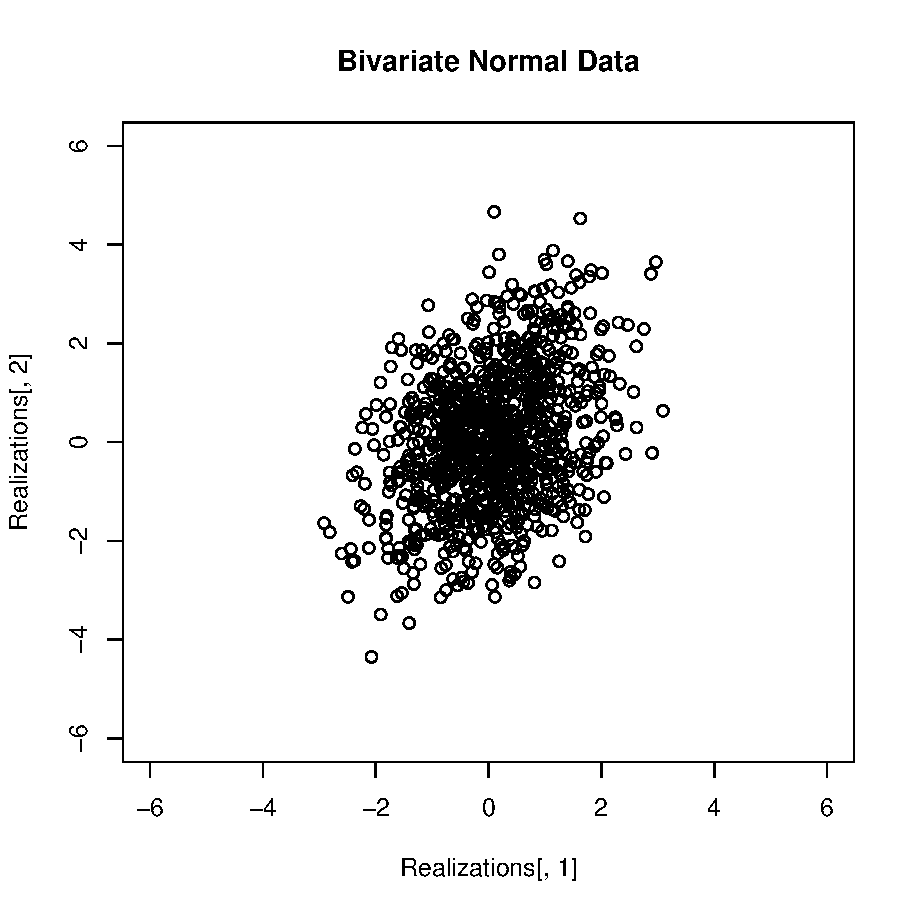
\includegraphics[width=15cm]{../Problem5.pdf}
\end{figure}
For this data we have the following as the means of the columns
\begin{lstlisting}[frame=trBL]
> apply(Realizations,2,mean)
[1] -0.03239635 -0.03260434
\end{lstlisting}
We then run the problem again and we have the following scatter-plot
\begin{figure}[ht!]
\centering
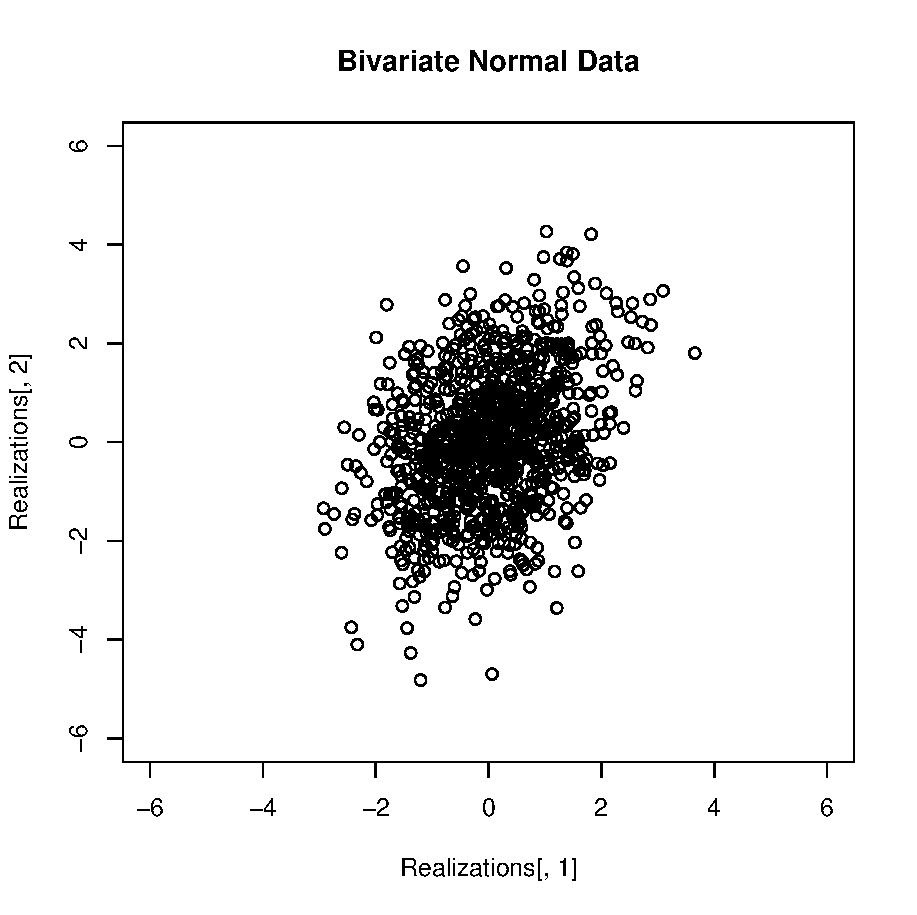
\includegraphics[width=15cm]{../Problem5Again.pdf}
\end{figure}
and for this we have the following as the means of the columns
\begin{lstlisting}[frame=trBL]
> apply(Realizations,2,mean)
[1] 0.01286922 0.03089901
\end{lstlisting}
As we see for the means, both are close to 0, and as we ran the code for a second time, we see that (perhaps by co-incidence) we have means closer, in magnitude, to 0.
\item[Problem 6]\hfill\\
Using \verb+rexp+ we see the syntax of inputs is \verb+rexp(n,1/mean)+, where n is the number of outcomes. So, for a mean of 1 and 50 outcomes, we can use \verb+rexp(50,1)+. Thus, to produce the sum, we would use 
\begin{lstlisting}[frame=trBL]
> sum(rexp(50,1))
\end{lstlisting}
To produce this sum 1000 times, we use the following loop
\begin{lstlisting}[frame=trBL]
realization<-rep(1,1000)
for( i in 1:1000){
	realization[i]<-sum(rexp(50,1))
}
\end{lstlisting}
Then using \verb+length+, we have the percentage of sums above 60
\begin{lstlisting}[frame=trBL]
> 100*length(which(realization>60))/length(realization)
[1] 8.8
\end{lstlisting}
Thus there are 8.8\% of the 1000 sums above 60.
\item[Problem 7]\hfill\\
To find the number of iterations it takes to find the sum of 50 realizations over 80, we run
\begin{lstlisting}[frame=trBL]
i<-0
testsum<80
while(testsum<80){
	testsum<-sum(rexp(50,1))
	i<-i+1
}
print(i)
\end{lstlisting}
Running this a few times, we require 1554 iterations, 16034 iterations, 3313 iterations to have the sum over 80.
\item[Problem 8]\hfill\\
Using the following code
\begin{lstlisting}[frame=trBL]
> X<-rnorm(1000,0,1)
> Y<-rnorm(1000,0,2)
> Z<-X+Y
> hist(Z)
> dev.print(device=pdf,"Problem8.pdf")
\end{lstlisting}
we have the following histogram
\begin{figure}
\centering
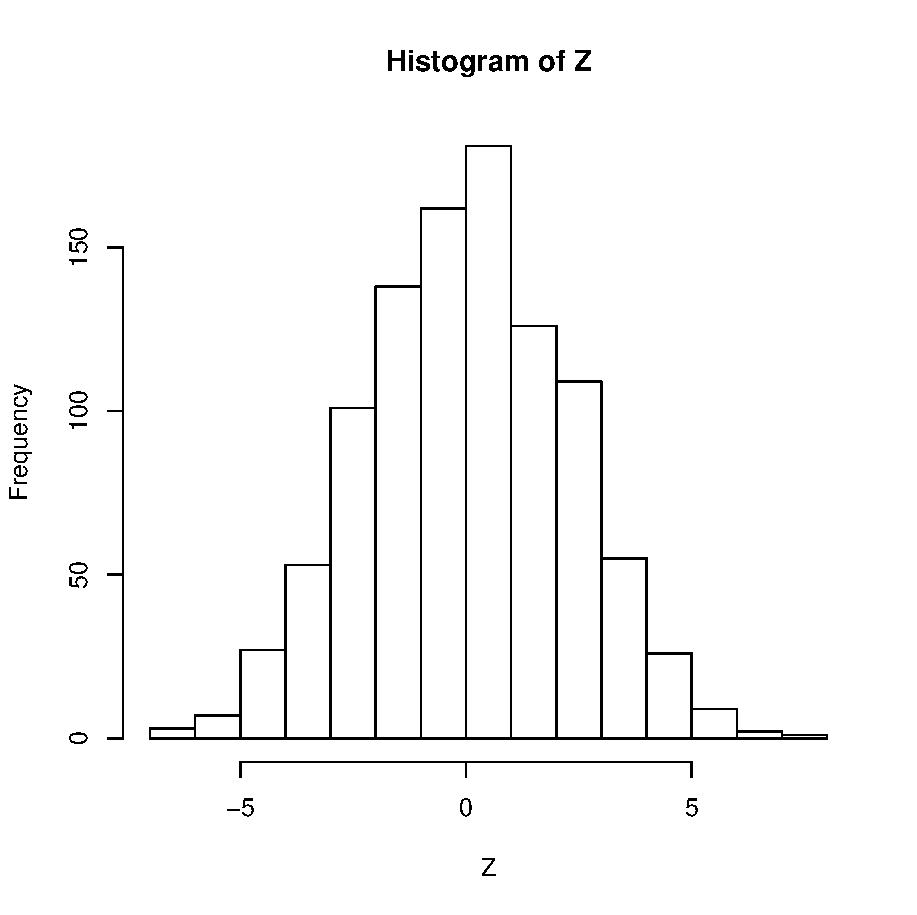
\includegraphics[width=15cm]{../Problem8.pdf}\caption{Problem 8 Plot}
\end{figure}
This plot seems to be a Normal distribution about 0.

\item[Problem 9]
Using the following code
\begin{lstlisting}[frame=trBL]
> X<-rnorm(1000,0,1)
> Y<-rnorm(1000,X,2)
> Z<-X+Y
> hist(Z)
> dev.print(device=pdf,"Problem9.pdf") 
\end{lstlisting}
we have the following plot.
\begin{figure}[ht!]
\centering
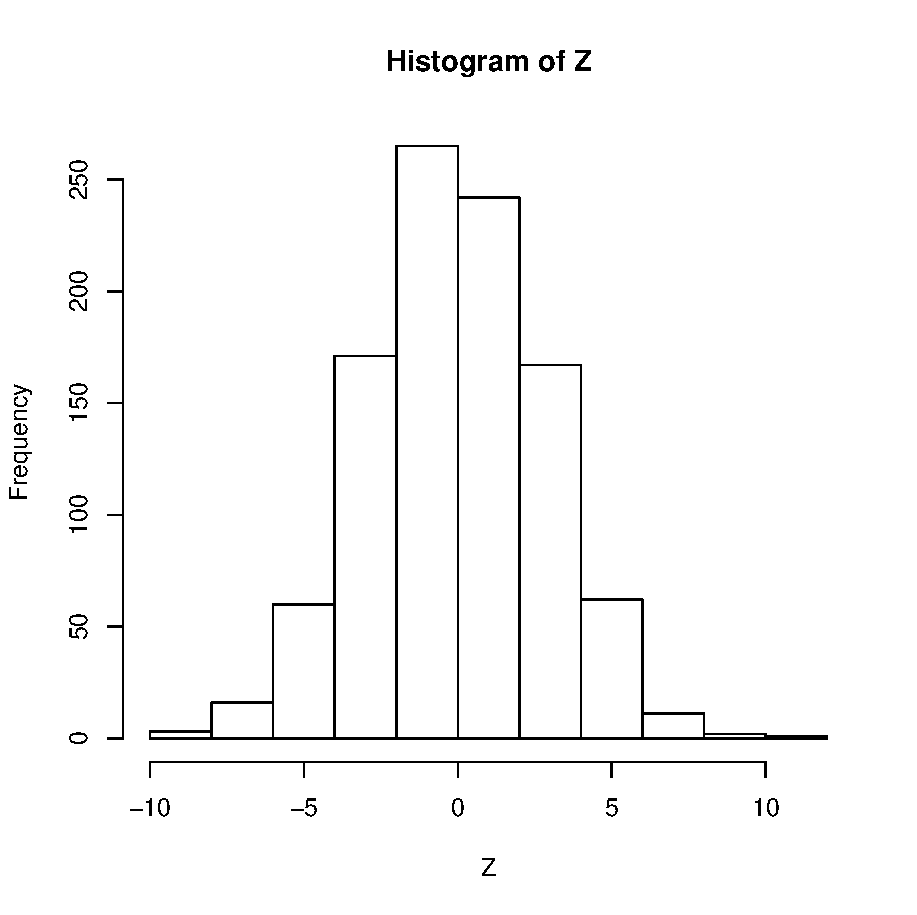
\includegraphics{../Problem9.pdf}\caption{Problem 9 Plot}
\end{figure}
Which still looks Normal about 0, but shows a bit of being skewed. 
\end{description}
\end{document}